% Figure blocks and captions, called from the body files.

\newcommand{\figSchematic}{%
\begin{figure*}[t]
\centering
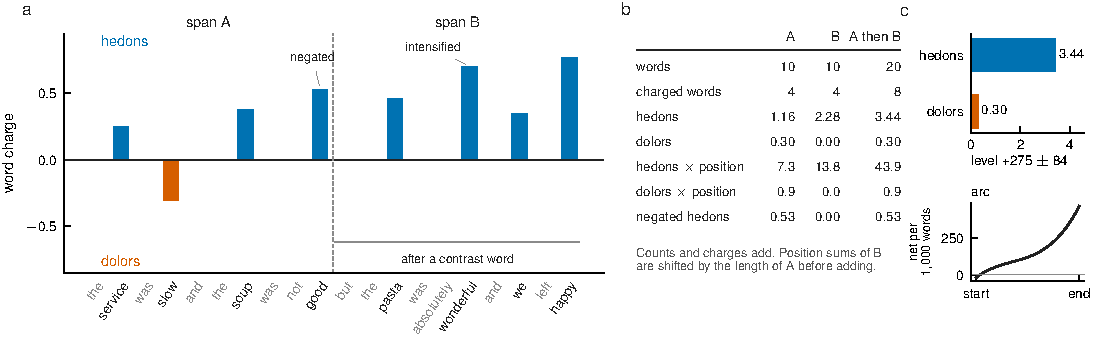
\includegraphics[width=\textwidth]{figures/fig1_schematic.pdf}
\caption{\textbf{Charge, signature, merge, readouts.} \textbf{a}, Two sentences scored word by word. Bars above the line are hedons, bars below are dolors; grey words are buffer words and carry no charge. \emph{Good} sits inside the reach of \emph{not}, \emph{wonderful} follows an intensifier, and the second sentence follows a contrast word. \textbf{b}, Entries of the signature of each sentence and of the two read as one text, obtained by merging and equal to a single pass over both. \textbf{c}, Readouts of the merged signature: totals, the level with its standard error (shipped $a$ and $\kappa$ for the level), and the cubic arc of net charge over relative position.}
\label{fig:schematic}
\end{figure*}}

\newcommand{\figAccuracy}{%
\begin{figure*}[t]
\centering
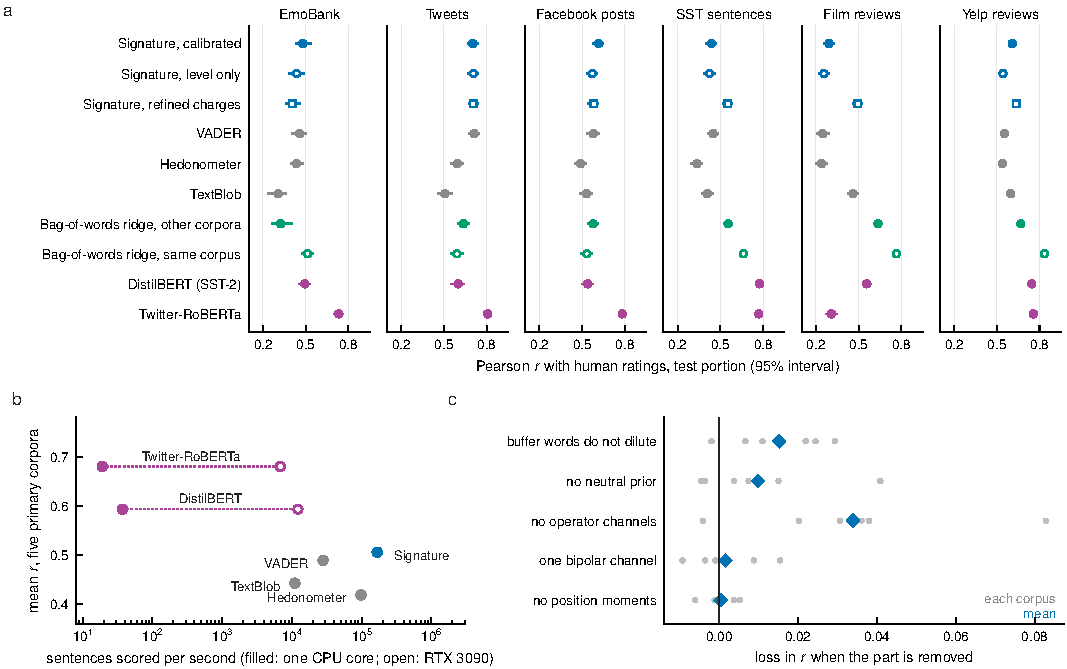
\includegraphics[width=\textwidth]{figures/fig2_accuracy.pdf}
\caption{\textbf{Agreement with human ratings, and cost.} \textbf{a}, Pearson $r$ between score and human rating on the held-out test portion of each corpus, with 95\% bootstrap intervals. Blue: readouts of the signature, with constants fitted on the other five corpora (filled circle, calibrated valence; open circle, level; square, calibrated valence with refined word charges). Grey: lexicon methods. Green: bag-of-words ridge regression trained on the other five corpora (filled) or on the same corpus (open). Purple: transformer classifiers. \textbf{b}, Mean $r$ over the five corpora with continuous human ratings against sentences scored per second on one CPU core. \textbf{c}, Loss in $r$ when one part of the signature is removed and the constants are refitted.}
\label{fig:accuracy}
\end{figure*}}

\newcommand{\figPosition}{%
\begin{figure*}[t]
\centering
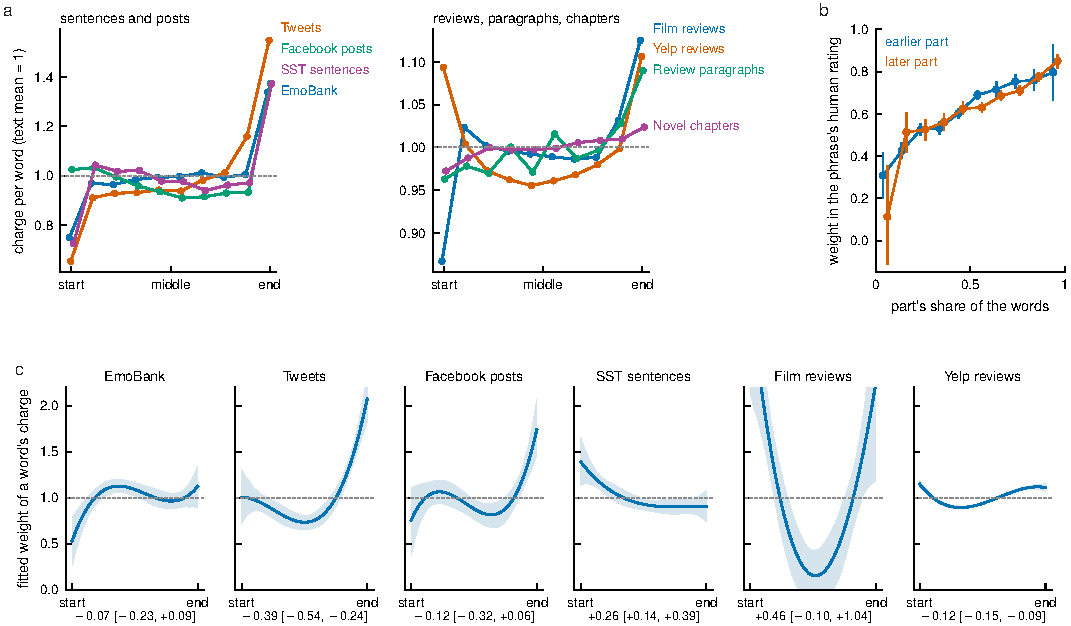
\includegraphics[width=\textwidth]{figures/fig3_position.pdf}
\caption{\textbf{Feeling is not front-loaded.} \textbf{a}, Charge per word in each tenth of a text, relative to the text's mean, for texts of ten or more words. \textbf{b}, Weights of the earlier and the later part in a regression of a phrase's human rating on the human ratings of its two parts, for binary nodes of the Stanford Sentiment Treebank (95\% intervals, sentences resampled). \textbf{c}, Position kernel fitted against human ratings in each corpus: the weight given to a word's charge as a function of its relative position, with 95\% bands. Below each panel, the mean weight over the first third minus the mean over the last third. The kernel for whole film reviews is poorly determined.}
\label{fig:position}
\end{figure*}}

\newcommand{\figDilution}{%
\begin{figure*}[t]
\centering
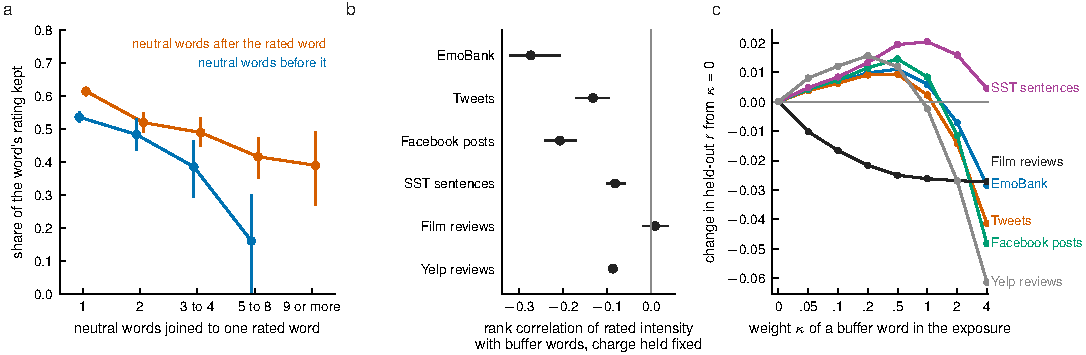
\includegraphics[width=\textwidth]{figures/fig4_dilution.pdf}
\caption{\textbf{Neutral words dilute a rating when they follow it.} \textbf{a}, Human phrase ratings from the Stanford Sentiment Treebank. A phrase with a clear rating is joined to a neutral phrase; the vertical axis is the share of the first phrase's rating that the joined phrase keeps, by the number of neutral words and their side (95\% intervals). \textbf{b}, Partial rank correlation between rated intensity and the number of buffer words in a text, with total charge held fixed. \textbf{c}, Change in held-out $r$ as the weight $\kappa$ of a buffer word in the exposure moves away from zero, with coefficients refitted at each value.}
\label{fig:dilution}
\end{figure*}}

\newcommand{\figBook}{%
\begin{figure*}[t]
\centering
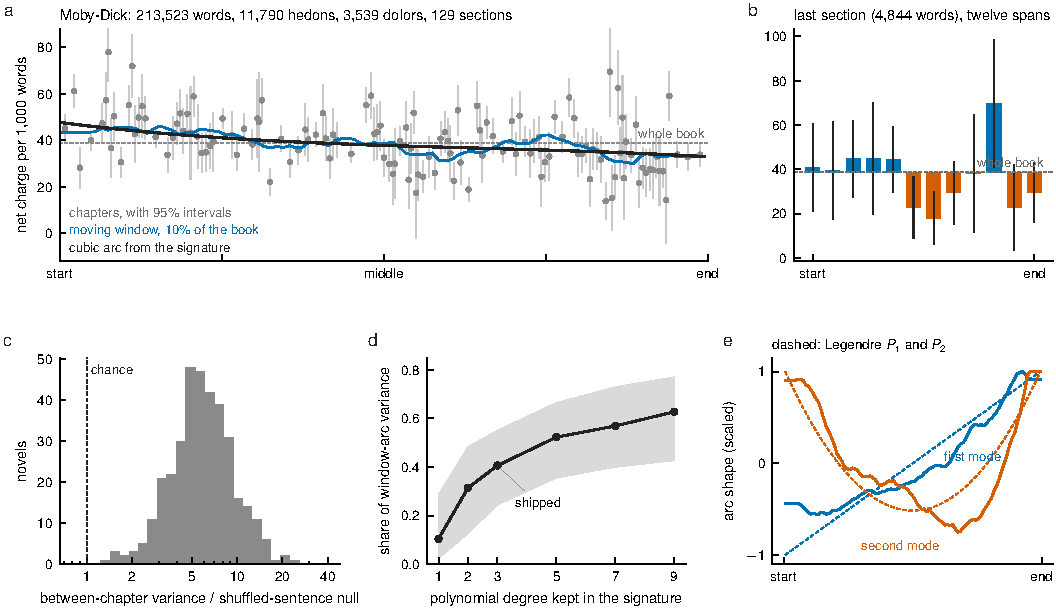
\includegraphics[width=\textwidth]{figures/fig5_book.pdf}
\caption{\textbf{A novel at three scales from one pass.} \textbf{a}, \emph{Moby-Dick}: density of each chapter with 95\% intervals from the word-level standard error, the cubic arc read from the book's signature, and a moving-window arc for comparison. \textbf{b}, The final chapter cut into twelve runs of sentences, each read from two rows of the prefix table; bars show the difference from the whole book's density. \textbf{c}, Between-chapter variance of density relative to its value when sentences are shuffled across chapters, for \nNovels{} novels. \textbf{d}, Share of the variance of the moving-window arc captured by the polynomial arc, by the highest degree kept (median and interquartile range). \textbf{e}, The two leading modes of variation among the novels' window arcs, with the first two Legendre polynomials.}
\label{fig:book}
\end{figure*}}

\newcommand{\figAggregation}{%
\begin{figure*}[t]
\centering
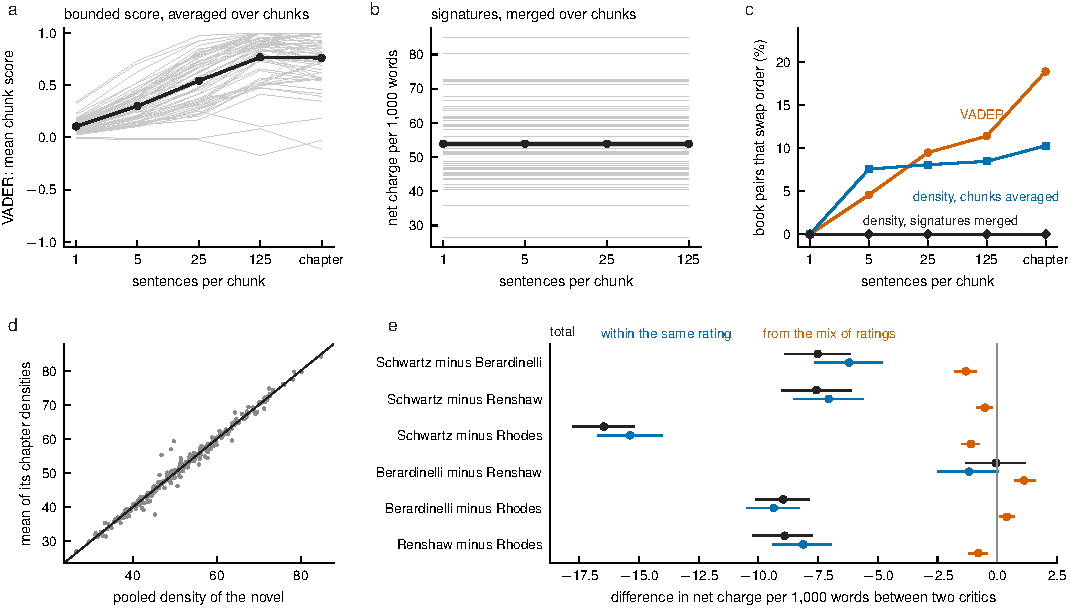
\includegraphics[width=\textwidth]{figures/fig6_aggregation.pdf}
\caption{\textbf{Averaging depends on the cut; merging does not.} \textbf{a}, Book score for \vaderBooks{} novels computed as the mean VADER compound score over chunks of a given number of sentences (grey, each novel; black, mean). \textbf{b}, Density of the same novels from signatures of the same chunks, merged. \textbf{c}, Share of pairs of novels whose order changes relative to one-sentence chunks. \textbf{d}, Pooled density of each of \nNovels{} novels against the mean of its chapter densities (per 1,000 words). \textbf{e}, Differences in density between four film critics, split into the part within the same rating and the part due to the mix of ratings (95\% intervals).}
\label{fig:aggregation}
\end{figure*}}

\newcommand{\figMachine}{%
\begin{figure*}[t]
\centering
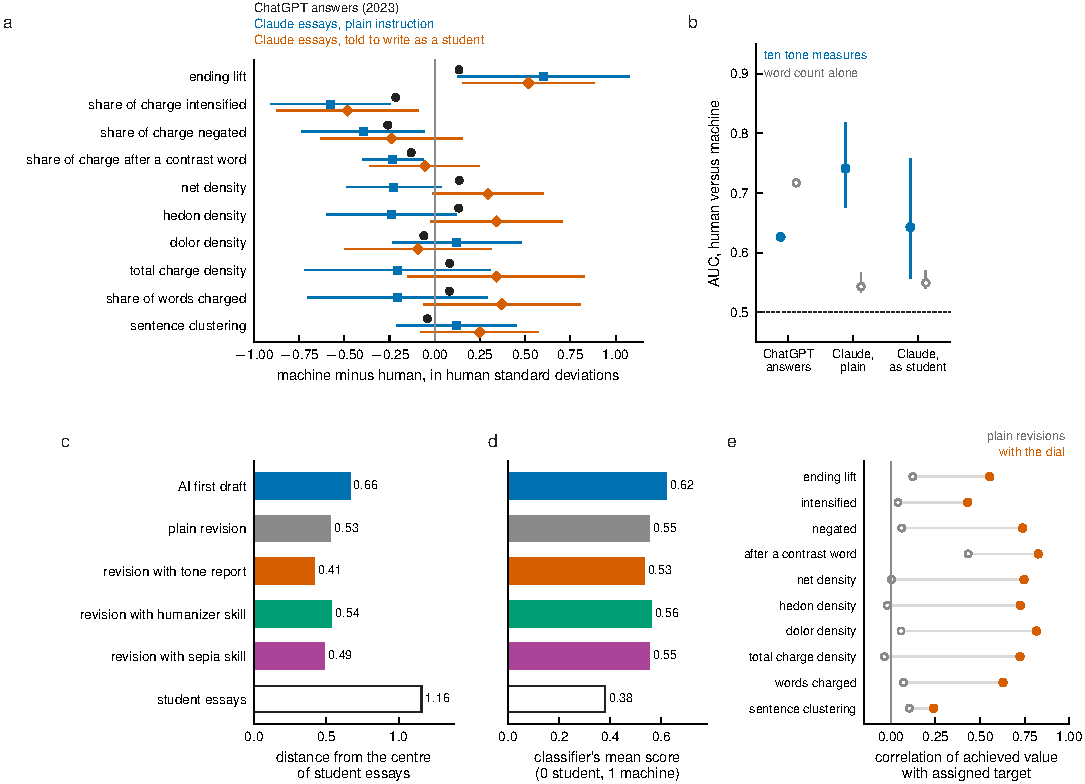
\includegraphics[width=\textwidth]{figures/fig7_machine.pdf}
\caption{\machineCaption}
\label{fig:machine}
\end{figure*}}

\newcommand{\figExtended}{%
\begin{figure*}[t]
\centering
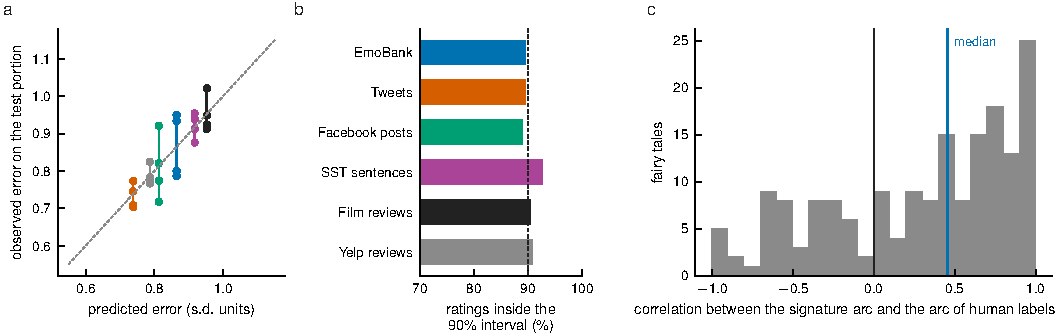
\includegraphics[width=\textwidth]{figures/figE1_uncertainty_tales.pdf}
\caption{\textbf{Error against exposure, and arcs of fairy tales.} \textbf{a}, Error of the calibrated score against human ratings on each test portion, in quartiles of exposure, against the error predicted by a variance model with a term that shrinks with exposure; the fitted model kept no such term, and observed error does not fall with exposure. \textbf{b}, Share of ratings inside the 90\% interval implied by the fitted variance. \textbf{c}, Correlation between the cubic arc of a tale's merged signature and the cubic arc of its sentence labels from two human annotators, for \nTales{} fairy tales.}
\label{fig:extended}
\end{figure*}}
